%\documentclass[10pt, twocolumn]{article}
%\documentclass[11pt]{article}
% \documentclass[twocolumn,showpacs,preprintnumbers,amsmath,amssymb,prl, superscriptaddress]{revtex4}
%\documentclass[twocolumn, preprintnumbers,amsmath,amssymb,prd, superscriptaddress]{revtex4}
\documentclass[preprintnumbers,amsmath,amssymb,prd,superscriptaddress]{revtex4}
%\documentclass[10pt, preprint,showpacs,preprintnumbers,amsmath,amssymb, superscriptaddress]{revtex4}
%\documentclass[11pt, prd,preprintnumbers,amsmath,amssymb, superscriptaddress]{revtex4}
%\documentclass[11pt, prd,preprintnumbers, amsmath,amssymb, superscriptaddress, nofootinbib, hyperref]{revtex4}

\usepackage{latexsym}
\usepackage{amssymb}
\usepackage{epsfig,amsmath,graphics}
\usepackage{epstopdf}
\usepackage{verbatim}
\usepackage{wasysym}
\usepackage{hyperref}
\usepackage{feynmp-auto} % feynman diagrams
%\usepackage{subfig}
\usepackage[utf8]{inputenc}
\usepackage{xpatch}
\usepackage{xcolor}
\usepackage{mathtools}
\hypersetup{
    colorlinks,
    linkcolor={red!80!black},
    citecolor={green!60!black},
    urlcolor={blue!60!black}}
\usepackage{appendix}

\newcommand{\Ez}{\mathcal{E}_0}
\newcommand{\Eboom}{\mathcal{E}_\text{boom}}
\newcommand{\OO}{\mathcal{O}}
\newcommand{\LL}{\mathcal{L}}
\newcommand{\HH}{\mathcal{H}}
\newcommand{\TeV}{\text{TeV}}
\newcommand{\GeV}{\text{GeV}}
\newcommand{\MeV}{\text{MeV}}
\newcommand{\keV}{\text{keV}}
\newcommand{\rad}{\text{rad}}
\newcommand{\cm}{\text{cm}}
\newcommand{\bn}{\text{b}} % barn
\newcommand{\mbn}{\text{mb}} % \millibarn
\newcommand{\angstrom}{\buildrel _{\circ} \over {\mathrm{A}}}
\newcommand{\pslash}{p\hspace{-0.070in}/\,}
\newcommand{\Mpl}{M_{\text{pl}}}
\newcommand{\ket}[1]{\ensuremath{\left|#1\right>}}
\newcommand{\bra}[1]{\ensuremath{\left<#1\right|}}
\newcommand{\braket}[2]{\ensuremath{\left<#1|#2\right>}}
\newcommand{\x}[1]{\ensuremath{\text{#1}}} % text mode shortcut
\newcommand{\kin}{\text{kin}}
\newcommand{\xmin}{\text{min}}
\newcommand{\xmax}{\text{max}}
\newcommand{\ion}{\text{ion}}
\newcommand{\TF}{\text{TF}}
\newcommand{\LPM}{\text{LPM}}
\newcommand{\el}{\text{el}}
\newcommand{\inel}{\text{inel}}
%Large Parentheses
\def\r{\right)}
\def\l{\left(}

\newcommand{\overbar}[1]{\mkern 1.5mu\overline{\mkern-1.5mu#1\mkern-1.5mu}\mkern 1.5mu}

\begin{document}

%\preprint{APS/123-QED}

\title{White Dwarfs as Dark Matter Detectors}

\author{Peter W. Graham}
\affiliation{Stanford Institute for Theoretical Physics, Department of Physics,
Stanford University, Stanford, CA, 94305}

\author{Ryan Janish}
\affiliation{Berkeley Center for Theoretical Physics, Department of Physics,
University of California, Berkeley, CA 94720, USA}

\author{Vijay Narayan}
\affiliation{Berkeley Center for Theoretical Physics, Department of Physics,
University of California, Berkeley, CA 94720, USA}

\author{Surjeet Rajendran}
\affiliation{Berkeley Center for Theoretical Physics, Department of Physics,
University of California, Berkeley, CA 94720, USA}

\author{Paul Riggins}
\affiliation{Berkeley Center for Theoretical Physics, Department of Physics,
University of California, Berkeley, CA 94720, USA}

\begin{abstract}
Dark matter that is capable of sufficiently heating a local region in a white dwarf will trigger runaway fusion and ignite a type Ia supernova.
This was originally proposed in~\cite{Graham:2015apa} and used to constrain primordial black holes which transit and heat a white dwarf via dynamical friction.
In this paper, we consider dark matter (DM) candidates that heat through the production of high-energy standard model (SM) particles, and show that such particles will efficiently thermalize the white dwarf medium and ignite supernovae.
Based on the existence of long-lived white dwarfs and the observed supernovae rate, we derive new constraints on ultra-heavy DM which produce SM particles through DM-DM annihilations, DM decays, and DM-SM scattering interactions in the stellar medium. 
As a concrete example, we rule out supersymmetric Q-ball DM in parameter space complementary to terrestrial bounds.
It is also intriguing that the DM-induced ignition discussed in this work provide an alternative mechanism of triggering supernovae from sub-Chandrasekhar Mass progenitors.
\end{abstract}

\maketitle

%%%%%%%%%%%%%%%%%%%%%%%%%%%%%%%%%%%%%%%%%%%%%%%%%%%%%%%%%%%%%%%%
\section{Introduction}
\label{sec:intro}
Identifying the nature of dark matter (DM) remains one of the clearest paths beyond the Standard Model (SM) and it is thus fruitful to study the observable signatures of any yet-allowed DM candidate.
Many terrestrial direct detection experiments are designed to search for DM, e.g.~\cite{Akerib:2016vxi, Agnese:2017njq}, yet these lose sensitivity to heavier DM due to its diminished number density.
Even for a strongly-interacting candidate, if the DM mass is above $\sim 10^{22}~\GeV$ a detector of size $\sim (100~\text{m})^2$ will register fewer than one event per year.
While these masses are large compared to those of fundamental particles, it is reasonable to suppose that DM may exist as composite states just as the SM produces complex structures with mass much larger than fundamental scales (e.g., you, dear reader).
Currently there is a wide range of unexplored parameter space for DM candidates less than $\sim 10^{48}~\GeV$, above which the DM will have observable gravitational microlensing effects~\cite{Griest:2013aaa}.
For such ultra-heavy DM, indirect signatures in astrophysical systems are a natural way forward.
One such signal, proposed by~\cite{Graham:2015apa}, is that DM can trigger runaway fusion and ignite type Ia supernovae (SN) in sub-Chandrasekhar white dwarf (WD) stars.

In addition to constraining the properties of DM, this raises the intriguing possibility that DM-induced runaway fusion is responsible for a fraction observed astrophysical transients. 
The progenitors of type Ia SN are not fully understood~\cite{
Maoz:2012}, and recent observations of sub-Chandrasekhar~\cite{Scalzo:2014sap, Scalzo:2014wxa}, hostless~\cite{McGee:2010}, and unusual type Ias~\cite{Foley:2013} suggest that multiple progenitor systems and ignition mechanisms are operative.
Other suspected WD thermonuclear events, such as the Ca-rich transients~\cite{Kasliwal:2012}, are also poorly understood. 
While mechanisms for these events have been proposed~\cite{Woosley1994,Fink:2007fv,Pakmor:2013wia,Sell:2015rfa}, the situation is yet unclear and it is worthwhile to consider new sources of thermonuclear ignition. 

Runaway thermonuclear fusion requires both a heating event and the lack of significant cooling which might quench the process.
The WD medium is particularly suited to this as it is dominated by degeneracy pressure and undergoes minimal thermal expansion, which is the mechanism that regulates fusion in main sequence stars.
Thermal diffusion is the primary cooling process in a WD and it can be thwarted by heating a large enough region.
The properties of a localized heating necessary to trigger runaway fusion were computed in~\cite{Woosley}.
Consequently, it was realized~\cite{Graham:2015apa} that if DM is capable of sufficiently heating a WD in this manner, it will result in a SN with sub-Chandrasekhar mass progenitor.
This was used to constrain primordial black holes which transit a WD and cause heating by dynamical friction, although the authors of~\cite{Graham:2015apa} identify several other heating mechanisms which may be similarly constrained.

In this paper, we examine DM candidates with non-gravitational interactions that cause heating through the production of SM particles.
An essential ingredient in this analysis is understanding the length scales over which SM particles deposit energy in a WD medium.
We find that most high energy particles thermalize rapidly, over distances shorter than or of order the critical size for fusion. 
Particle production is thus an effective means of igniting WDs. 
Constraints on these DM candidates come from either observing specific, long-lived WDs or by comparing the measured rate of type Ia SN with that expected due to DM.
It is important to note that these constraints are complementary to direct searches---it is more massive DM that is likely to trigger SN, but also more massive DM that has low terrestrial flux.
The WD detector excels in this regime due to its large surface area $\sim (10^4~\text{km})^2$, long lifetime $\sim \text{Gyr}$, and galactic abundance.
We demonstrate these constraints for generic classes of DM models that produce SM particles via DM-SM scattering, DM-DM collisions, or DM decays, and consider the significantly enhanced constraints for DM that is captured in the star.
As a concrete example we consider ultra-heavy Q-ball DM as found in supersymmetric extensions of the SM. 

The rest of the paper is organized as follows.
We begin in Section~\ref{sec:boomreview} by reviewing the mechanism of runaway fusion in a WD.
In Section~\ref{sec:smheating} we study the heating of a WD due to the production of high-energy SM particles.
Detailed calculations of the stopping of such particles are provided in Appendix~\ref{sec:wdpdg}.
In Section~\ref{sec:dmignition} we parameterize the explosiveness and event rate for generic classes of DM-WD encounters, and in Section~\ref{sec:constraints} we derive schematic constraints on such models.
The details of DM capture in a WD are reserved for Appendix~\ref{sec:capture}.
Finally we specialize to the case of Q-balls in Section~\ref{sec:qballs}, and conclude in Section~\ref{sec:discussion}.

%%%%%%%%%%%%%%%%%%%%%%%%%%%%%%%%%%%%%%%%%%%%%%%%%%%%%%%%%%%%%%%%
\section{White Dwarf Runaway Fusion}
\label{sec:boomreview}
We first review the conditions for which a local energy deposition in a WD results in runaway fusion.
Any energy deposit will eventually heat ions within some localized region---parameterize this region by its linear size $L_0$, total kinetic energy $\Ez$ and typical temperature $T_0$.
These scales evolve in time, but it will be useful to describe a given heating event by their initial values.

The fate of a heated region is either a nonviolent diffusion of the excess energy across the star, or a runaway fusion chain-reaction that destroys the star.
The precise outcome depends on $L_0$, $\Ez$ and $T_0$.
There is a critical temperature $T_f$, set by the energy required for ions to overcome their mutual Coulomb barrier, above which fusion occurs.
For carbon burning, $T_f \sim \MeV$~\cite{Gasques:2005ar}.
Any heated region $T_0 > T_f$ will initially support fusion, although this is not sufficient for runaway as cooling processes may rapidly lower the temperature below $T_f$.
This cooling will not occur if the corresponding timescale is larger than the timescale at which fusion releases energy.
Cooling in a WD is dominated by thermal diffusion, and the diffusion time increases as the size of the heated region.
However, the timescale for heating due to fusion is independent of region size.
Thus, for a region at temperature $\gtrsim T_f$, there is a critical size above which the heated region does not cool but instead initiates runaway.
For a region at the critical fusion temperature $T_f$, we call this critical size the \emph{trigger size} $\lambda_T$.
The value of $\lambda_T$ is highly dependent on density, and in a WD is set by the thermal diffusivity of either photons or degenerate electrons.
This critical length scale has been computed numerically in~\cite{Woosley} for a narrow range of WD densities and analytically scaled for other WD masses in~\cite{Graham:2015apa}.
As in~\cite{Graham:2015apa}, we will restrict our attention to carbon-oxygen WDs in the upper mass range $\sim 0.85 - 1.4 ~M_{\astrosun}$ (these will yield the most stringent constraints on DM).
This corresponds to a central number density of ions $n_\text{ion} \sim 10^{30} - 10^{32} ~\cm^{-3}$ and a trigger size of $\lambda_T \sim 10^{-3} - 10^{-5} ~\text{cm}$.

If a heated region is smaller than the trigger size, its thermal evolution is initially dominated by diffusion.
However, this will still result in runaway fusion if the temperature is of order $T_f$ by the time the region diffuses out to the trigger size.
For our purposes it is more natural to phrase this in terms of the total energy $\Ez$ deposited during a heating event.
Of course, the relation between energy $\Ez$ and temperature $T_0$ depends on the rate at which WD constituents---ions, electrons, and photons---thermalize with each other within the region size $L_0$.
Given that the different species thermalize rapidly, the excess energy required to raise the temperature to $T_f$ in a volume $V$ is given by a sum of their heat capacities
\begin{equation}
\label{eq:heatcapacity}
  \frac{\Ez}{V} \gtrsim \int_0^{T_f} dT (n_\text{ion} + n_e^{2/3} T + T^3),
\end{equation}
where $n_e$ is the number density of electrons.
Note that we use the heat capacity of a degenerate gas of electrons, since the Fermi energy $E_F \gtrsim \MeV$ for the densities we consider.
The minimum energy deposit necessary to trigger runaway fusion is simply
\begin{align}
\label{eq:Eboom}
\Eboom &\sim \lambda_T^3 (n_\text{ion} T_f + n_e^{2/3} T_f^2 + T_f^4) \\
&\approx 10^{16} - 10^{23} ~\GeV. \nonumber
\end{align}
$\Eboom$ varies with $\lambda_T$ over the range of WD densities and is plotted in Figure~\ref{fig:Eboom}.
Thus for a heating event characterized by its $L_0$, $\Ez$, and $T_0 \gtrsim T_f$, there is an \emph{ignition condition}:
\begin{align}
    \label{eq:energy_boom_condition}
    \Ez \gtrsim
    \Eboom \cdot \text{max}\left\{1, \frac{L_0}{\lambda_T}\right\}^3.
\end{align}
Any $\Ez$ satisfying this condition is minimized for $L_0$ less than the trigger size, where it is also independent of the precise value of $L_0$.
For broader deposits, the necessary energy is parametrically larger than $\Eboom$ by a volume ratio $(L_0/\lambda_T)^3$.
As a result, understanding the $L_0$ for different kinds of heating events in a WD is critical to determining whether or not they are capable of destroying the star.

\begin{figure}
\includegraphics[scale=.3]{Eboom.pdf}
\caption{The minimum energy deposit~\eqref{eq:Eboom} necessary to trigger runaway fusion, based on numerical results for $\lambda_T$~\cite{Woosley} and the WD mass-density relation~\cite{cococubed}}.
\label{fig:Eboom}
\end{figure}


%%%%%%%%%%%%%%%%%%%%%%%%%%%%%%%%%%%%%%%%%%%%%%%%%%%%%%%%%%%%%%%%
\section{Particle Heating of White Dwarfs}
\label{sec:smheating}
We address now the possibility of DM heating the WD medium via the production of SM particles.
The critical quantity is the length scale over which such SM particles heat the medium---this scale determines their efficiency in triggering runaway fusion as described by condition \eqref{eq:energy_boom_condition}.
Note that this is a question of purely SM physics.
The unknown physics of DM will serve only to set the initial properties of the SM particles.

One may have expected that efficient heating occurs only for a limited range of SM species and energies, thus restricting the set of DM candidates capable of producing SN.
However, we find that SM particles tend to efficiently heat the WD regardless of species or energy---the length scale of heating is typically less than or of order the trigger size $\lambda_T$, and is never parametrically larger.
This is accomplished primarily through hadronic showers initiated by collisions with carbon ions.
In some cases electromagnetic shower processes are important, however at high energies these are suppressed by density effects and photons/electrons are dominated by hadronic interactions.
These interactions rapidly stop high-energy particles due to the logarithmic nature of showers, converting them into a cloud of low-energy particles which efficiently heat the WD medium through elastic scatters.
In this light, the WD operates analogously to a particle detector, including hadronic and electromagnetic ``calorimeter'' components.
Runaway fusion provides the necessary amplification to convert a detected event into a recordable signal, in this case a violent SN.

In the remainder of this section we present the above heating process in detail.
We summarize the dominant source of energy loss and the resulting stopping lengths $\lambda$ for SM particles of incident kinetic energy $\epsilon$, approximated by $\sim \frac{\epsilon}{dE/dx}$, where $dE/dx$ is the stopping power in the WD medium.
These are plotted in Figures \ref{fig:SPhighEM}, \ref{fig:SPlowEM}, \ref{fig:SPhighHad}, and \ref{fig:SPlowHad}.
A detailed treatment of the stopping powers is reserved for Appendix \ref{sec:wdpdg}. 
We will consider incident light hadrons, photons, electrons, and neutrinos---as we are concerned with triggering runaway fusion, we restrict our attention to energies $\epsilon \gg T_f \sim \text{MeV}$.
A cartoon schematic for this flow of energy deposition for the various incident particles is given in Figure \ref{fig:heating-cartoon}.
%Note that an explosive heating event may either produce a few high-energy particles or a large number of lower energy particles.
%These scenarios can have very different heating lengths, and we will distinguish between them when applicable.

\subsection{High-Energy Showers}

\paragraph{Hadronic Showers.}
Incident hadrons with kinetic energy larger than the nuclear binding scale $E_\text{nuc} \sim 10~\MeV$ will undergo violent inelastic collisions with carbon ions resulting in an $\OO(1)$ number of secondary hadrons.
This results in a roughly collinear shower of hadrons which ends when the constituents reach an energy $\sim E_\text{nuc}$.
This occurs over a shower length
\begin{align}
\label{eq:hadlength}
  X_\text{had} \sim l_\text{inel} \log\l\frac{\epsilon}{E_\text{nuc}}\r
  \approx 10^{-6} ~\text{cm} \l\frac{10^{32}~\text{cm}^{-3}}{n_\text{ion}}\r
\end{align}
where $l_\text{inel}$ is the mean free path for nuclear scatters, set by $\sigma_\text{inel} \approx 100 ~\text{mb}$, and we have taken the logarithm to be $\sim 10$.
The shower terminates into an exponential number of $\sim 10~\MeV$ hadrons with roughly equal fractions of pions, protons, and neutrons.
For a more detailed discussion of hadronic showers, see Appendix~\ref{sec:nuclear}.
Note that neutral pions of energy $10 - 100 ~\text{MeV}$ have a decay length to photons of order $\delta_{\pi^0} \sim 10^{-6} ~\text{cm}$.
Hadronic showers will therefore generate an electromagnetic component carrying an $\OO(1)$ fraction of the energy.

\paragraph{Photonuclear and Electronuclear Showers.}
The LPM effect (see next section) ensures that hadronic interactions become important at sufficiently high energies even for electrons and photons.
Photons can interact hadronically via quark-antiquark pairs and directly induce hadronic showers off ions.
The only quantitative difference between these showers and purely hadronic ones is that they require a slightly longer distance to initiate.
Roughly, the photonuclear cross section is suppressed relative to the hadronic inelastic cross section by a factor of $\alpha$ required to produce a quark-antiquark pair.
This gives a photon range
\begin{align}
\label{eq:photonuclength}
  \lambda_{\gamma A} \sim \frac{l_\text{inel}}{\alpha}
  \approx 10^{-5} ~\text{cm} \l\frac{10^{32}~\text{cm}^{-3}}{n_\text{ion}}\r.
\end{align}
Note that $\lambda_{\gamma A}$ is the distance to begin a hadronic shower, whereas the shower itself extends a distance $X_\text{had}$.

In the regime of strong LPM suppression, high-energy electrons will also initiate hadronic showers through virtual photons. 
This process is best described as a continuous energy loss of the electron into minimal $\sim 10 ~\MeV$ hadronic showers.  
The electronuclear stopping length is 
\begin{align}
\label{eq:electronuclength}
  \lambda_{eA}
  \approx 10^{-4} ~\text{cm} \l\frac{10^{32}~\text{cm}^{-3}}{n_\text{ion}}\r.
\end{align}
This is suppressed by an additional factor of $\alpha$ relative to the photonuclear interaction, however a full calculation also yields an $\OO(10)$ logarithmic phase-space enhancement.
For electron energies greater than $\sim 10^6 - 10^8 ~\GeV$ (depending on the WD density), electronuclear stopping even dominates over the bremsstrahlung of real photons that then interact hadronically. 

\paragraph{Electromagnetic Showers.}
Of course, electrons and photons also shower through successive bremsstrahlung and pair-production interactions.
An EM shower proceeds until a critical energy $\sim 100 ~\MeV$ set by the scale at which these radiative processes become subdominant to Coulomb and Compton scattering.
Below this scale radiation can still be important, though EM showers do not occur.
Note that bremsstrahlung and pair-production are strictly forbidden for incident energies below the electron Fermi energy.

At sufficiently high electron/photon energies and nuclear target densities, EM showers are elongated due to the ``Landau-Pomeranchuk-Migdal" (LPM) effect.
High-energy radiative processes necessarily involve small momentum transfers to nuclei. 
These soft virtual photons cannot be exchanged with only a single ion, but rather interact simultaneously with multiple ions. 
This generates a decoherence, suppressing bremsstrahlung/pair-production above an energy $E_\text{LPM}$ which scales inversely with density:
\begin{align}
    E_\text{LPM} \approx 1~\MeV
    \l \frac{10^{32}~\text{cm}^{-3}}{n_\text{ion}} \r
\end{align}
The corresponding shower lengths are
\begin{align}
  X_\text{EM} &\approx X_0 \cdot \begin{cases}
  \l \frac{\epsilon}{E_\text{LPM}} \r^{1/2} & \epsilon > E_\text{LPM} \\
  \;\;\;\;\;\, 1 & \epsilon < E_\text{LPM}
  \end{cases}
\end{align}
where
\begin{align}
  X_0 &\approx 10^{-7} ~\text{cm}
  \l\frac{10^{32}~\text{cm}^{-3}}{n_\text{ion}}\r.
\end{align}
See Appendix~\ref{sec:emshowers} for further details. 
At the highest WD densities radiative processes are always LPM-suppressed, while at lower densities we observe both regimes.
In high-density WDs, EM showers completely carry the energy of $\sim 10^2 - 10^4~\text{MeV}$ electrons and photons. 
The lower end of this range corresponds to the scale at which elastic scatters dominate, and the upper end corresponds to the scale at which photonuclear interactions dominate. 
%In low-density WDs, the latter will occur at an energy $\sim 10^6 ~\GeV$. 

\paragraph{Neutrino-induced Showers}
Neutrinos scatter off ions with a cross section that increases with energy.
In these interactions, an $\OO(1)$ fraction of the neutrino energy is transferred to the nucleus with the rest going to produced leptons \cite{Formaggio:2013kya}---this is sufficient to start a hadronic shower.
At an energy of $\sim 10^{11} ~\GeV$, neutrino-nuclear cross section is determined \cite{Formaggio:2013kya} to be $\sim 10^{-32} ~\cm^2$, which we will conservatively take as an estimate for even higher energies.
This gives a distance of order $\sim \text{meter}$ for a neutrino to initiate a hadronic shower.
While it is much too large to efficiently heat a WD via the release of multiple neutrinos, the neutrino mean free path is simply the displacement for a single high-energy neutrino to begin a shower of size $X_\text{had}$---this is qualitatively similar to the photonuclear length \eqref{eq:photonuclength}. 
As such, a single ultra-high energy neutrino released in the WD can efficiently heat the star. 

\subsection{Low-Energy Elastic Heating}

The showers of high-energy particles described above terminate in a cloud of low-energy $\epsilon \sim 10~\MeV$ neutrons, protons, and charged pions, and $\epsilon \sim 100~\MeV$ electrons and photons.
Of course, particles at these energies may also be directly produced by the DM.
At these energies, Coulomb, Compton, and elastic nuclear scatters dominate and eventually lead to the thermalization of ions.
The stopping powers for these processes are calculated in the Appendix. 

\paragraph{Nucleons and Pions.}
Neutrons and neutral pions are the simplest species we consider, interacting at low-energies only through elastic nuclear scatters characterized by a cross section $\sigma_\text{el} \approx \text{b}$, enhanced from the inelastic interaction by a factor of $\sim 10$. 
Note that the mass hierarchy between these particles and the ions requires $\sim 10 - 100$ scatters to transfer the hadron's energy in the form of a random-walk.
This elastic heating range is approximately
\begin{align}
 \lambda_\text{el} &\approx
 10^{-7} ~\text{cm} \l\frac{10^{32}~\text{cm}^{-3}}{n_\text{ion}}\r,
\end{align}
and is always less than the trigger size.
Note that this may or may not be shorter than the neutral pion decay length $\delta_{\pi^0}$, depending on the WD density.
Low-energy neutrons thus always provide efficient heating, low-energy neutral pions provide efficient heating at high densities, and the effectiveness of neutral pions at low densities depends on the stopping of $\approx 70~\text{MeV}$ photons.
We now turn to charged hadrons, which are subject to Coulomb interactions with ions and electrons as well as elastic nuclear scatters similar to their neutral brethren.
At energies $\epsilon \lesssim 10~\MeV$, scattering off electrons is in fact the least dominant of these processes, contrary to the behavior of terrestrial detectors.
This is due to the significant Pauli-blocking of electron interactions near the Fermi energy $E_F \sim 1-10~\MeV$.
Low-energy charged hadrons will thus predominantly lose energy through elastic nuclear scatters or in a small range of energies, Coulomb scatters off ions---either way, both interactions length scales are well below the trigger size and transfer energy to ions. 
In the context of a hadronic shower, the final-state hadrons are $\sim 10~\MeV$ nucleons and pions, with each species carrying an $\OO(1)$ fraction of the initial energy.
These products will thermalize within a trigger size and thus hadronic showers are also an efficient heating mechanism.

\paragraph{Electrons and Photons.}
As shown in Figures \ref{fig:SPhighEM} and \ref{fig:SPlowEM}, electron stopping at low energy is dominated by bremsstrahlung and photon stopping by Compton scatters.
Thus, at these energies electrons and photons first thermalize into a compact electromagnetic ``gas" of size $X_\text{EM} < \lambda_T$. 
This gas cools and diffuses to larger length scales, eventually allowing subdominant processes to thermalize carbon ions.
The details of this evolution depend on the initial EM gas temperature $T$, which is set by the total SM energy released by the DM.
If the gas is below $10~\MeV$ before the photonuclear scale, the dominant process will be Coulomb scattering of hot electrons off WD ions.
We have checked that this is the case for any EM cloud formed from the final-state products of high-energy electromagnetic showers. 
Note that for temperatures $T$ less than the Fermi energy, the electrons are partially degenerate and heating proceeds via the thermal tail with kinetic energies $\epsilon \sim E_F + T$.
We calculate this stopping length is roughly of order but slightly larger than the trigger size.
The fact that this length scale is larger than the trigger size simply means that constraints relying on this specific heating process will have some volume dilution, increasing the necessary energy deposit according to~\eqref{eq:energy_boom_condition}.
If instead the gas remains above $10~\MeV$ by the time it has diffused to a size $\lambda_{\gamma A}$, the photons in the gas will efficiently thermalize ions via photonuclear showers and subsequent nuclear elastic heating (see discussion above). 

%%%%%%%%%%%%%%%%%%%%%%%%%%%%%%%%%%%%%%%%%%%%%%%%%%%%%%%%%%%%%%%%
\section{Dark Matter-Induced Ignition}
\label{sec:dmignition}
Any DM interaction that produces SM particles in a WD has the potential to ignite the star, provided that sufficient SM energy is produced.
The distribution in space, momentum, and species of these SM products is dependent on unknown DM physics and is needed to determine the rate of DM-induced ignition.
This can be done precisely for a specific DM model, as we do for Q-balls in Section~\ref{sec:qballs}.
In this Section, however, we study some general features of DM-WD encounters involving DM that possesses interactions with itself and the SM.
We collect below the basic formulas relating DM model parameters to ignition criteria, SN rate, etc.

DM can generically heat a WD through three basic processes: DM-SM scattering, DM-DM collisions, and DM decays.
For ultra-heavy DM, these processes can be complicated events involving many (possibly dark) final states, analogous to the interactions of heavy nuclei.
In the case of DM-SM scattering, we consider both elastic and inelastic DM scatters off WD constituents, e.g. carbon ions. 
We classify DM candidates into three types according to the interaction that provides the dominant source of heating, and refer to these as scattering, collision, and decay candidates.
We also make the simplifying assumption that the above events are ``point-like", producing SM products in a localized region (smaller than the heating length) near the interaction vertex.
If this is not the case (as with very large Q-balls, see Section~\ref{sec:qballs}), then the same formalism applies but with the event size added to the stopping length.

The SN rate may be greatly enhanced if DM is captured in the star, so we also consider separately ``transiting DM" and ``captured DM".
In general, there is some loss of DM kinetic energy in the WD.
In the transit scenario, this energy loss is negligible and the DM simply passes through the star.
In the capture scenario, the energy loss is not directly capable of ignition but is sufficient to stop the DM and cause it to accumulate in the star.
Energy loss may be due to a variety of processes, but for simplicity we will focus on an DM-nuclei elastic scattering. 
Of course, due to the velocity spread of DM in the rest frame of a WD, there will necessarily be both transiting and captured DM populations in the star.

\subsection{DM Transit}

\paragraph{DM-SM Scattering.}
Runaway fusion only occurs in the degenerate WD interior where thermal expansion is suppressed as a cooling mechanism.
The outer layers of the WD, however, are composed of a non-degenerate gas and it is therefore essential that a DM candidate penetrate this layer in order to ignite a SN.
We parameterize this by a DM stopping power $(dE/dx)_\text{SP}$, the kinetic energy lost by the DM per distance traveled in the non-degenerate layer, and demand that
\begin{align}
\label{eq:CrustCondition}
  \left( \frac{d E}{d x} \right)_\text{SP} \ll
  \frac{m_\chi v^2_\text{esc}}{R_\text{env}}.
\end{align}

DM-SM scattering will result in a continuous energy deposit along the DM trajectory (if the interaction is rare enough for this not to be true, then the encounter is analogous to the case of DM decay).
This is best described by a linear energy transfer $(dE/dx)_\text{LET}$, the kinetic energy of SM particles produced per distance traveled by the DM.
If these products have a heating length $L_0$ then the energy deposit must at minimum be taken as the energy transferred along a distance $L_0$ of the DM trajectory.
Importantly, as per the ignition condition~\eqref{eq:energy_boom_condition}, such a deposition is \emph{less} explosive unless $L_0$ is smaller than the trigger size $\lambda_T$.
We thus consider the energy deposited over the larger of these two length scales.
Assuming the energy of the DM is roughly constant during this heating event, the ignition condition is:
\begin{align}
\label{eq:transitexplosion}
  \left( \frac{d E}{d x} \right)_\text{LET} \gtrsim
  \frac{\Eboom}{\lambda_T} \cdot \text{max}
  \left\{\frac{L_0}{\lambda_T}, 1 \right\}^2.
\end{align}
Note that the DM stopping power $(dE/dx)_\text{SP}$ and the linear energy transfer $(dE/dx)_\text{LET}$ are related in the case of elastic scatters, but in general the two quantities may be controlled by different physics.
In addition, a transit event satisfying condition~\eqref{eq:CrustCondition} will have negligible energy loss over the parametrically smaller distances $\lambda_T$ or $L_0$, validating~\eqref{eq:transitexplosion}.

The above condition sums the individual energy deposits along the DM trajectory as though they are all deposited simultaneously.
This is valid if the DM moves sufficiently quickly so that this energy does not diffuse out of the region of interest before the DM has traversed the region.
We therefore require that the diffusion time $\tau_\text{diff} \sim 10^{-12}~\text{s}$ across a heated region of size $L$ at temperature $T_f$ be larger than the DM crossing-time:
\begin{align}
  \tau_\text{diff} \sim \frac{L^2}{\alpha(T_f)} \gg
  \frac{L}{v_\text{esc}},
\label{eq:SlowDiffusion}
\end{align}
where $\alpha(T)$ is the temperature-dependent diffusivity, and the DM transits at the stellar escape velocity $v_\text{esc} \sim 10^{-2}$.
This condition is more stringent for smaller regions, so we focus on the smallest region of interest, $L = \lambda_T$.
Then~\eqref{eq:SlowDiffusion} is equivalent to demanding that the escape speed is greater than the conductive speed of the fusion wave front, $v_\text{cond} \sim \alpha(T_f) / \lambda_T$.
Numerical calculations of $v_\text{cond}$ are tabulated in~\cite{Woosley}, and indeed condition~\eqref{eq:SlowDiffusion} is satisfied for all WD densities.

The rate of transit events is directly given by the flux of DM through a WD
\begin{align}
  \Gamma_\text{trans} \sim
  \frac{\rho_{\chi}}{m_\chi} R_\text{WD}^2
  \l\frac{v_\text{esc}}{v_\text{halo}}\r^2 v_\text{halo},
\label{eq:TransitRate}
\end{align}
where $\rho_\chi$ is the DM density in the region of the WD, and $R_\text{WD}$ is the WD radius.
Here $v_\text{halo} \sim 10^{-3}$ is the virial velocity of our galactic halo.
Note the $(v_\text{esc}/v_\text{halo})^2 \sim 100$ enhancement due to gravitational focusing.

We will not consider here captured DM that heats the star via scattering events, as such heating will typically cause ignition before capture occurs.
However, it is possible to cause ignition after capture if the collection of DM leads to an enhanced scattering process.

\paragraph{DM-DM Collisions and DM Decays.}

For a point-like DM-DM collision or DM decay event releasing particles of heating length $L_0$, ignition will occur if the total energy in SM products satisfies condition~\eqref{eq:energy_boom_condition}.
Such an event will likely result in both SM and dark sector products, so we parameterize the resulting energy in SM particles as a fraction $f_\text{SM}$ of the DM mass.
For non-relativistic DM, the DM mass is the dominant source of energy and therefore $f_\text{SM} \lesssim 1$ regardless of the interaction details.
A single DM-DM collision or DM decay has an ignition condition:
\begin{equation}
\label{eq:coldecay}
  m_\chi f_\text{SM} \gtrsim \Eboom \cdot \text{max} \left \{\frac{L_0}{\lambda_T}, 1 \right \}^3.
\end{equation}
Thus the WD is sensitive to annihilations/decays of DM masses $m_\chi > 10^{16} ~\GeV$.

DM that is not captured traverses the WD in a time $t_\text{ff} \sim R_\text{WD}/v_\text{esc}$, and the rate of DM-DM collisions within the WD parameterized by cross-section $\sigma_{\chi \chi}$ is:
\begin{align}
  \Gamma^\text{ann}_\text{SN}
  \sim \l \frac{\rho_\chi}{m_\chi} \r^2 \sigma_{\chi \chi} \l \frac{v_\text{esc}}{v_\text{halo}}\r^3 v_\text{halo} R_\text{WD}^3.
  \label{eq:collisionDM}
\end{align}
Similarly the net DM decay rate inside the WD parameterized by a lifetime $\tau_\chi$ is:
\begin{align}
 \Gamma^\text{decay}_\text{SN}
   \sim \frac{1}{\tau_\chi} \frac{\rho_{\chi}}{m_\chi} \l \frac{v_\text{esc}}{v_\text{halo}}\r R_\text{WD}^3.
  \label{eq:decayDM}
\end{align}

\subsection{DM Capture}

\paragraph{Review of DM Capture.}

We first summarize the capture and subsequent evolution of DM in the WD, ignoring annihilations or decays---see Appendix~\ref{sec:capture} for details.
Consider a spin-independent, elastic scattering off carbon ions with cross section $\sigma_{\chi A}$.
The rate of DM capture in gravitating bodies is of course very well-studied~\cite{Press:1985ug, Gould:1987ir}.
However, this rate must be modified when the DM requires multiple scatters to lose the necessary energy for capture.
Ultimately, for DM massive enough to ignite and not ruled out by direct detection experiments,the capture rate is of the form
\begin{equation}
\Gamma_\text{cap} \sim \Gamma_\text{trans} \cdot \l n_\text{ion} \sigma_{\chi A} R_\text{WD} \frac{m_\text{ion} v_\text{esc}^2}{m_\chi v_\text{halo}^2} \r.
\end{equation}
Once DM is captured, it eventually thermalizes with the stellar medium to a velocity
\begin{equation}
  v_\text{th} \approx 10^{-11} \l \frac{m_\chi}{10^{16} ~\GeV}\r^{-1/2},
\end{equation}
and settles at the thermal radius
\begin{align}
  R_\text{th} \approx 0.1 ~\cm \l \frac{m_\chi}{10^{16} ~\GeV}\r^{-1/2}.
\end{align}
Note that all numerical quantities in this section are evaluated at a WD central density $n_\text{ion} \sim 10^{31}~\cm^{-3}$. 
DM thermalization proceeds in two stages.
Captured DM will initially be found on a large, bound orbit that decays after many transits of the WD until the orbital size is fully contained within the star.
This occurs after a time
\begin{equation}
\label{eq:thermalization1}
t_1 \approx 7\times 10^{16}~\text{s}
  \l \frac{m_\chi}{10^{16} ~\GeV} \r^{3/2}
  \l \frac{\sigma_{\chi A}}{10^{-35} ~\cm^2} \r^{-3/2}.
\end{equation}
The DM then completes many orbits within the star until its orbital size decays to the thermal radius.
This occurs after a time
\begin{equation}
\label{eq:thermalization2}
t_2  \approx 10^{14}~\text{s}\l \frac{m_\chi}{10^{16} ~\GeV} \r
  \l \frac{\sigma_{\chi A}}{10^{-35} ~\cm^2} \r^{-1}.
\end{equation}
Note that the difference in scalings between $t_1$ and $t_2$ is due to the fact that, while the two times are ultimately determined by scattering in the star, the dynamics of the settling DM are quite distinct in each case. 
For instance, $t_1$ is dominated by the time spent on the largest orbit outside the WD (which additionally depends on $\sigma_{\chi A}$) while $t_2$ is dominated by the time spent near the thermal radius. 
Subsequently the DM will begin steadily accumulating at $R_\text{th}$, with the possibility of self-gravitational collapse if the collected mass of DM exceeds the WD mass within this volume.
This occurs after a time
\begin{align}
\label{eq:tsg}
t_\text{sg} &\approx
  10^{9} ~\text{s} \l \frac{m_\chi}{10^{16} ~\GeV} \r^{-1/2}
  \l \frac{\sigma_{\chi A}}{10^{-35} ~\cm^2} \r^{-1}.
\end{align}
Of course, not all of these stages may be reached within the age of the WD $\tau_\text{WD} \sim 5 ~\text{Gyr}$.
The full time to collect and begin self-gravitating is $t_1 + t_2 + t_\x{sg}$.
Importantly, for DM masses $m_\chi > 10^{16} ~\GeV$ self-gravitation sets in instantly relative to thermalization.
This time is less than $\tau_\text{WD}$ if
\begin{equation}
\label{eq:settle}
\sigma_{\chi A} \gtrsim 10^{-35} ~\cm^2 \l \frac{m_\chi}{10^{16} ~\GeV} \r.
\end{equation}
Note that constraints from direct detection~\cite{Aprile:2017iyp} demand that the scattering cross section be sufficiently small
\begin{equation}
\label{eq:directdet}
\sigma_{\chi A} \lesssim 10^{-29} ~\cm^2 \l \frac{m_\chi}{10^{16} ~\GeV} \r.
\end{equation}
However \eqref{eq:directdet} is relaxed for $m_\chi \gtrsim 10^{22}~\GeV$, at which point direct detection experiments lack the necessary exposure to constrain the DM.  

At any point during the above evolution, captured DM has the potential to trigger a SN.
Of particular interest is the ability of DM to ignite a WD during self-gravitational collapse, either via annihilations or the formation of a black hole.
A collapse can release sufficient energy to trigger SN even with DM masses less than $10^{16} ~\GeV$.
However, such a process involves additional subtleties beyond the scope of this paper and is the focus of forthcoming work~\cite{us}.
In the following, we require that a single collision or decay is sufficient to ignite the star, and give only a quick assessment of collapse.

\paragraph{Captured DM-DM Collisions.}
We now turn to the rate of DM-DM collisions for captured DM.
Of course, the thermalizing DM constitutes a number density of DM throughout the WD volume.
Assuming the scattering cross section satisfies~\eqref{eq:settle} and~\eqref{eq:directdet}, the total rate of annihilations for this ``in-falling" DM is peaked near the thermal radius and is of order:
\begin{equation}
\label{eq:infall}
\Gamma_\text{infall} \sim \frac{(\Gamma_\text{cap} t_2)^2}{R_\text{th}^3} \sigma_{\chi \chi} v_\text{th}.
\end{equation}
If $\Gamma_\text{infall} t_2 > 1$, then a SN will be triggered by the in-falling DM population.
Otherwise if $\Gamma_\text{infall} t_2 < 1$, the DM will start accumulating at the thermal radius---since $t_\text{sg} \ll t_2$ for such heavy DM masses, there will be no collisions during this time and thus a collapse will proceed. 
As we will see, ignition of a WD during collapse is almost guaranteed unless $\sigma_{\chi \chi}$ is sufficiently small.
When the DM sphere is at a radius $r$, the rate of annihilations is
\begin{align}
\label{eq:collapse}
\Gamma_\text{collapse} &\sim \frac{(\rho_\text{WD} R_\x{th}^3/ m_\chi)^2}{r^3} \sigma_{\chi \chi} v_\chi, \\
 v_\chi &\sim \sqrt{\frac{G \rho_\text{WD} R_\text{th}^3}{r}}.
\end{align}
Here we have conservatively taken the number of collapsing particles to be the self-gravitational threshold---as mentioned in Appendix~\ref{sec:capture}, this is an underestimate for such ultra-heavy DM.
We also assume the timescale for collapse is set by the DM cooling rate and is thus related to $t_2$---see Appendix~\ref{sec:capture} for details.
Of course, there may be some stabilizing physics which prevents the DM from collapsing and annihilating below a certain radius, such as formation of a black hole or bound states.
To illustrate the stringent nature of the collapse constraint we will simply assume some benchmark stable radius, as in Figure~\ref{fig:capture-collision}. 
Note that if a single collision has not occurred during collapse, one may additionally examine annihilations of the subsequent in-falling DM down to the stable radius---for simplicity, we do not consider this scenario.

\paragraph{Captured DM Decays.}
Lastly, we compute the rate of decays for captured DM, which is simply proportional to the number of DM particles in the WD available for decay at any given instance.
In the transit scenario~\eqref{eq:decayDM}, this number is $\sim \Gamma_\text{trans} t_\text{ff}$.
In the capture scenario, this number is instead determined by the thermalization time within the WD:
\begin{equation}
\Gamma_\text{decay} \sim  \frac{1}{\tau_\chi} \Gamma_\text{cap} t_2,
\label{eq:decayDMcap}
\end{equation}
conservatively assuming that after a thermalization time, the DM quickly collapses and stabilizes to an ``inert" core incapable of further decay.
If this is not the case, then the captured DM decay rate is given by replacing $t_2 \to \tau_\text{WD}$ in~\eqref{eq:decayDMcap}.


%%%%%%%%%%%%%%%%%%%%%%%%%%%%%%%%%%%%%%%%%%%%%%%%%%%%%%%%%%%%%%%%
\section{Dark Matter Constraints}
\label{sec:constraints}
We now constrain some simplified models of DM which will ignite a WD via one of the processes parameterized in Section \ref{sec:dmignition}.
First, however, we review how WD observables constrain DM candidates capable of triggering SN.

\subsection{Review of WD Observables}
Following the discussion of \cite{Graham:2015apa}, our constraints come from (1)~the existence of heavy, long-lived white dwarfs, or (2)~the measured type 1a SN rate.
The typical age of a WD is of order the age of the universe $\sim \text{Gyr}$.
RX~J0648.04418 is a nearby star and one of the heavier known WDs, with a mass $\sim 1.25 ~M_{\astrosun}$ \cite{Mereghetti:2013nba} and local dark matter density which we will take to be $\rho_\chi \sim 0.4 ~\GeV/\text{cm}^3$.
Of course, this is not the only known heavy WD---the Sloan Digital Sky Survey \cite{SDSS} has found $20+$ others.
 % https://heasarc.gsfc.nasa.gov/db-perl/W3Browse/w3hdprods.pl
The NuStar collaboration has also recently uncovered evidence for the likely existence of $\sim 1.25 ~M_{\astrosun}$ WDs in the galactic center \cite{NuStar}, where it is estimated that $\rho_\chi \sim 10^3 ~\text{GeV}/\text{cm}^3$ \cite{Nesti:2013uwa}.
Such heavy candidates are particularly suited for our constraints as the energy deposit necessary to trigger SN $\Eboom$ is a decreasing function of WD mass.
However, less dense white dwarfs are significantly more abundant in the galaxy.
Thus, even if a sufficiently massive DM is unable to trigger a violent heating event within the lifetime of a WD, it could still ignite enough lighter WDs to affect the measured SN rate of $\sim $ 0.3 per century.
The DM-induced SN rate is estimated using the expected number of white dwarfs per galaxy $\sim 10^{10}$ and their mass distribution \cite{SDSS}.
Simulations indicate that only WD masses heavier than $\sim 0.85 ~M_{\astrosun}$ will result in optically visible SN \cite{Graham:2015apa}.
Therefore, most of the stars exploded in this manner will be in the mass range $\sim 0.85 - 1 ~M_{\astrosun}$, resulting in weaker SN than expected of typical Chandrasekhar mass WDs.

To summarize, a bound on DM parameters can be placed if either a single explosive event occurs during the lifetime of an observed star such as RX~J0648.04418, or the SN rate due to such DM events throughout the galaxy exceeds the measured value.
Note that for low-mass WDs dominated by photon diffusion, $\Eboom$ is a strong function of WD density.
In \cite{Graham:2015apa} the central WD density is used to constrain black hole transits with the justification that the density is nearly constant for much of the star.
The average density for WDs is typically a factor $\sim 10^{-2} - 10^{-1}$ less than the central density, although it is found that the WD density only changes by an $\OO(1)$ fraction from the central value up to a distance $\sim R_\text{WD}/2$ \cite{Chandrasekhar}.
Therefore the central density is a valid approximation as long as we consider heating events within this ``modified" WD volume.
For simplicity, we employ this approach.

\subsection{Transit Constraints}
\label{sec:TransitConstraints}

In order to constrain a DM model through its transit interaction with a WD, we require that it satisfy the boom condition \eqref{eq:transitexplosion}.
This is given in terms of an LET, which parameterizes the ability for DM to release sufficient energy to the star in the form of SM particles.
$(dE/dx)_\text{LET}$ for any realistic DM model would necessarily involve a sum over stellar targets along with species that could be produced, as well as an integral over the produced particle spectrum.
However, we will consider a simplified interaction in which $\sigma_{Ni\epsilon}$ denotes the cross-section for DM to scatter off a stellar constituent (e.g. ions), producing $N$ particles of SM species $i$ and individual energy $\epsilon$.
If this were the only available channel for the DM to deposit energy, then the LET could be written as
\begin{align}
\label{eq:schematicLET}
  \left( \frac{d E}{d x} \right)_\text{LET} = n_\text{ion} \sigma_{Ni\epsilon} N\epsilon.
\end{align}
The heating length for such a DM-SM scattering interaction is computed in Section~\ref{sec:smheating}.

Additionally, consider the case that the LET $(dE/dx)_\text{LET}$ and DM stopping power $(dE/dx)_\text{SP}$ are equal---that is, the DM loses kinetic energy at the same rate as energy is deposited to the WD.
While such a statement is certainly not true for all DM models (such as the Q-ball, which liberates binding energy rather than transferring kinetic energy), it provides a useful benchmark to express constraints.
It is interesting to note that in this case combining the transit explosion condition \eqref{eq:transitexplosion} with $\eqref{eq:schematicLET}$ yields a lower bound on DM mass such that the DM is able to both penetrate the envelope \emph{and} trigger an explosion:
\begin{align}
\label{eq:transitmass}
m_\chi > \Eboom \l \frac{R_\text{envelope}}{\lambda_T} \r \l \frac{\rho_\text{envelope}}{\rho_\text{central}} \r \frac{1}{v_\text{esc}^2}.
\end{align}
For the typical parameters of a $1.25 ~M_{\astrosun}$ WD we find that the DM mass must be greater than $\sim 10^{28} ~\GeV$ to ensure a penetrating and explosive transit, taking the density of the WD envelope $\rho_\text{envelope}$ to be a nominal $\OO(10^{-3})$ fraction of the central density $\rho_\text{central}$~\cite{KippenhahnWeigert}.
In other words, if \eqref{eq:transitmass} were violated then the DM interaction is either not strong enough to ignite the WD or is so strong that the DM cannot penetrate the envelope without losing appreciable kinetic energy.
We reiterate, however, that this bound is only applicable when the energy input to the WD is chiefly coming from the DM kinetic energy, rather than binding energy or other sources.

With the above schematic for a DM transit, we use the rates and heating lengths computed in previous sections to constrain the parameter $\sigma_{Ni\epsilon}$ as a function of DM mass $m_\chi$.
This is done in Figure \ref{fig:transitclasses} using the different classes of observation available and for representative choices of $\epsilon$ and SM species $i$ released.



\subsection{Collision and Decay Constraints}
\label{sec:CollisionConstraints}

In order to constrain a DM model through its annihilations or decays within a WD, we require that it satisfy the boom condition \eqref{eq:coldecay}.
Consider a simplified interaction where an annihilation or decay releases $N$ particles of SM species $i$ and individual energy $\epsilon$.
If we assume a fractional parameter $f_\text{SM}=1$, this corresponds to the entire mass of DM being converted into SM products $i$, each with energy $m_\chi/N$.
These will deposit their energy and thermalize ions within a distance described in Section \ref{sec:smheating}.

With this schematic for DM-DM collisions, we use the rates and heating lengths computed in previous sections to constrain the cross section $\sigma_{\chi \chi}$ as a function of $m_\chi$ using the different classes of observation available and for representative choices of $f_\text{SM}$ and SM species $i$ released.
This is done in Figure \ref{fig:collisionclasses} for the wind scenario and Figure \ref{fig:collisionclassescap} for the capture scenario.
The constraints obtained by considering multiple collisions are shown in Figure \ref{fig:multiplecollision}. 
In a similar manner, we constrain the lifetime $\tau_\chi$ as a function of $m_\chi$ in Figures \ref{fig:decayclasses} and \ref{fig:collisionclassescap}.

\emph{Complementary Limits}~~It is important to note that there are additional limits on DM interactions of this kind, complementary to the limits placed from WDs.
For instance, DM can annihilate or decay into ultra-high energy particles within our galactic halo and therefore contribute to the cosmic ray flux seen in terrestrial air shower detectors.
As cosmic rays of energy greater than $\sim 10^{12} ~\GeV$ have not yet been observed \cite{ThePierreAuger:2015rha, AbuZayyad:2012ru}, this places a concrete limit on DM interaction parameters $\sigma_{\chi \chi}$ and $\tau_\chi$ which involve the release of such ultra-high energy particles.
In theory, a constraint may also be placed on lower-energy SM products from DM annihilations or decays, which would provide an additional source for the measured cosmic ray flux, although such a detailed analysis is beyond the scope of this work.

The cosmic ray constraint on DM is derived by requiring that the expected time for an event to strike earth is less than the lifetime of the detector $\sim 10 ~\text{yr}$.
For a cosmic ray detector with area $ \sim (50~\text{km})^2$ \cite{ThePierreAuger:2015rha}, we find that the cosmic ray bounds are weaker than the WD bounds except in the DM decay ``wind scenario", where the cosmic rays bounds are comparable within a couple orders of magnitude to those due to the observation of a local WD.
This coincidence is simply a consequence of the similar ``space-time volumes" of the two systems.
A cosmic ray detector sees events within a space-time volume $\sim (R_\text{det}^2 R_\text{halo} \times 10 ~\text{yr})$ which is comparable to the WD space-time volume for decay events $\sim (R_\text{WD}^3 \times 10^9 ~\text{yr}\times 10)$, including the factor of 10 gravitational enhancement.

In addition, there are various cosmological bounds on DM interactions.
By requiring that the galactic halo has not diminished by more than an $\OO(1)$ factor during its lifetime, we constrain $\sigma_{\chi \chi}/m_\chi \lesssim \text{barn}/\GeV$, regardless of the precise details of the collision.
This is similar in magnitude to the DM self-interaction bounds from colliding galaxy clusters \cite{Randall:2007ph}.
The cosmological bound on DM lifetime $\tau_\chi \gtrsim 100 ~\text{Gyr}$ is also independent of the nature of the decay products (see \cite{Poulin:2016nat} for details).
Since the limits imposed by the WD scale as $\sigma_{\chi \chi} \propto m_\chi^2$ and $\tau_\chi \propto m_\chi^{-1}$, there will necessarily be a sufficiently large DM mass for which the above cosmological considerations are the more stringent constraints on its interactions.
This occurs for DM masses $m_\chi \sim 10^{25} - 10^{30} ~\GeV$.

We now turn towards constraints on DM-DM collisions in the capture scenario.
We do not show the bounds that can be placed if $m_\chi > \Eboom$ and a single collision or decay is capable of blowing up the star. 
These are obviously more stringent than that of the wind scenario---for decays, it is simply enhanced by a numerical factor $\sim 10^{5}$. 
In Figure \ref{fig:multicapture}, we derive the constraints on $\sigma_{\chi \chi}$ from the focusing of multiple collisions during gravitational collapse due of DM in the star.
Bounds are from the observation of a single $1.25 ~ M_{\astrosun}$ in our local DM density. 
The results of Figure \ref{fig:multicapture} are valid for any SM annihilation products which deposit their energy compactly upon release within the trigger size $\lambda_T$.

%%%%%%%%%%%%%%%%%%%%%%%%%%%%%%%%%%%%%%%%%%%%%%%%%%%%%%%%%%%%%%%%
\section{Q-balls}
\label{sec:qballs}
% !TEX root = wd-full.tex

Having derived constraints on generic models of ultra-heavy DM, we turn towards a concrete example.
In various supersymmetric extensions of the SM, non-topological solitons called Q-balls can be produced in the early universe~\cite{Coleman:1985ki, Kusenko:1997si}.
If these Q-balls were stable, they would comprise a component of the DM today.
For gauge-mediated models with flat scalar potentials, the Q-ball mass and radius are given by
\begin{equation}
\label{eq:Qballprop}
M_Q \sim m_S Q^{3/4}, ~~~ R_Q \sim m_S^{-1} Q^{1/4},
\end{equation}
where $m_S$ is related to the scale of supersymmetry breaking, and $Q$ is the global charge of the Q-ball---in our case, baryon number.
The condition $M_Q/Q < m_p$ ensures that the Q-ball is stable against decay to nucleons.
When a baryonic Q-ball interacts with a nucleon, it induces the dissociation of the nucleon and absorbs its baryonic charge.
During this proton decay-like process, excess energy of order $\Lambda_\text{QCD}$ is released via the emission of 2--3 pions~\cite{Kusenko:1998}.
We assume that for each Q-ball inelastic collision, there is equal probability to produce $\pi^0$ and $\pi^\pm$ under the constraint of charge conservation.
The cross section for this interaction is approximately geometric
\begin{align}
\sigma_Q \sim \pi R_Q^2,
\end{align}
and thus grows with increasing $Q$.
Note that a sufficiently massive Q-ball will become a black hole if $R_Q \lesssim G M_Q$.
In the model described above, this translates into a condition $(M_\text{pl}/m_S)^4 \lesssim Q$.

We now determine the explosiveness of a Q-ball transit.
This process is described by a linear energy transfer
\begin{equation}
\label{eq:QballLET}
\l\frac{dE}{dx}\r_\text{LET} \sim n_\text{ion} \sigma_Q N_\pi \epsilon,
\end{equation}
where the nuclear interaction results in $N_\pi \approx 30$ pions released, each with kinetic energy $\epsilon \approx 500 ~\text{MeV}$.
These pions induce hadronic showers which terminate in low-energy hadrons that rapidly transfer their energy to ions via elastic scatters, as discussed in Section~\ref{sec:smheating}.
The pions have a heating length $X_\text{had} \lesssim \lambda_T$; however, we will see the Q-ball has a finite size $R_Q \gtrsim X_\text{had}$ in the region we are able to constrain.
So, as mentioned in Section~\ref{sec:dmignition}, we take the heating length to be $L_0 \sim R_Q + X_\text{had} \sim R_Q$.
The ignition condition is then given by equations~\eqref{eq:transitexplosion} and~\eqref{eq:QballLET}:
\begin{equation}
 R_Q^2 \gtrsim \frac{1}{n_\text{ion}} \frac{\Eboom}{\lambda_T}
 \; \xmax\left \{ \frac{R_Q}{\lambda_T}, 1\right\}^2
 \l \frac{1}{10~\GeV} \r.
\end{equation}
This implies $\sigma_Q \gtrsim 10^{-12} ~\text{cm}^2$ is sufficient to ignite a $1.25 ~M_{\astrosun}$ WD, which corresponds to a charge $Q \gtrsim 10^{42} ~(m_S/\text{TeV})^4$.
Note that for sufficiently large $Q$, the radius will grow larger than $\lambda_T$.
This situation still results in ignition, however, as the energy $\sim 10~\GeV$ released per ion is much larger than the $\sim \MeV$ needed per ion for fusion.
Note finally that the Q-ball interaction described above results in minimal slowing for Q-balls this massive, so transits will easily penetrate the non-degenerate WD envelope~\eqref{eq:CrustCondition}.

The existing limits on Q-balls primarily come from Super-Kamiokande and air fluorescence detectors of cosmic rays (OA, TA)~\cite{Dine:2003ax}.
However, the constraints that come from considering the ignition of WDs are in a fundamentally new and complementary region of parameter space.
These are plotted in Figure~\ref{fig:Qballconstraint}.
We have also included the constraints that result from gravitational heating of a WD during a Q-ball transit, as in~\cite{Graham:2015apa}.

\begin{figure}
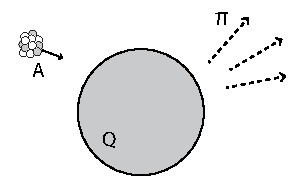
\includegraphics[scale=1.0]{qball-cartoon.pdf}
\caption{Interaction of a baryonic Q-ball with a nucleus $A$. The Q-ball destroys the nucleus and absorbs its baryonic charge, while the excess energy is radiated into roughly $A$ outgoing pions of energy $\Lambda_\text{QCD}$.}
\label{fig:qball-cartoon}
\end{figure}

\begin{figure}
\includegraphics[scale=.35]{Qballconstraint.pdf}
\caption{
Constraints on Q-ball DM.
Bounds come from demanding that the Q-ball interaction during a DM transit is capable of igniting WDs, occurring at a rate large enough to either ignite a single observed $1.25~M_{\astrosun}$ WD in its lifetime (WD in local DM density is blue shaded) or exceed the measured SN rate in our galaxy.
Also shown is the corresponding constraint from gravitational heating of WDs (orange shaded), and existing limits from terrestrial detectors (red)~\cite{Dine:2003ax}.}
\label{fig:Qballconstraint}
\end{figure}


%%%%%%%%%%%%%%%%%%%%%%%%%%%%%%%%%%%%%%%%%%%%%%%%%%%%%%%%%%%%%%%%
\section{Discussion}
\label{sec:discussion}
The detection of ultra-heavy DM is an open problem which will likely require a confluence of astrophysical probes.
Here we present a guide to constraining these candidates through DM-SM scatters, DM-DM annihilations, and DM decays inside a WD that release sufficient SM energy to trigger runaway fusion.
In particular, we calculate the energy loss of high-energy particles due to SM interactions within the WD medium and determine the conditions for which a general energy deposition will heat a WD and ignite SN.
Ultra-heavy DM that produces greater than $10^{16}~\GeV$ of SM particles in a WD is highly constrained by the existence of heavy WDs and the measured SN rate.
The formalism provided will enable WDs to be applied as detectors for any DM model capable of heating the star through such interactions. 
We have done so for baryonic Q-balls, significantly constraining the allowed parameter space in a complementary way to terrestrial searches. 

We have explored briefly the application of this WD instability to self-gravitational collapse of DM cores, which has very interesting possibilities. 
The decay or annihilation of DM which is captured by a WD and forms a self-gravitating core is highly constrained for DM with mass greater than $10^{16}~\GeV$.
In addition, such collapsing cores can provide enough heating via multiple annihilations to ignite the star for much smaller DM masses than those considered here, e.g.~$10^7~\GeV$, and can induce SN through other means such as the formation and evaporation of mini black holes. 
These will be addressed in future work~\cite{us}.  

Finally, in addition to the constraints mentioned above, the general phenomenology of these DM-induced runaways will be the ignition of sub-Chandrasekhar mass WDs, possibly with no companion star present.
Some of the mechanisms considered above are also likely to initiate fusion far from the center of the star. 
This is in contrast with conventional single-degenerate and double-degenerate mechanisms, which require a companion star and ignite fusion near the center of a super-Chandrasekhar mass WD~\cite{Maoz:2012}.  
This raises the tantalizing possibility that DM encounters with WDs provide an alternative explosion mechanism for type Ia SN or similar transient events, and that these events may be distinguishable from conventional explosions. 
Understanding and searching for possible distinguishing features of DM-induced events is an important follow-up work. 

%%%%%%%%%%%%%%%%%%%%%%%%%%%%%%%%%%%%%%%%%%%%%%%%%%%%%%%%%%%%%%%%
\begin{appendices}
\renewcommand{\thesubsection}{\arabic{subsection}}
\section{Particle Stopping in a White Dwarf}
\label{sec:wdpdg}
Here we provide a more detailed analysis of the stopping power (energy loss per distance traveled) of high-energy SM particles in a carbon-oxygen WD due to strong and electromagnetic interactions.
We consider incident electrons, photons, pions, and nucleons with kinetic energy greater than an $\MeV$.

%%%%%%%%%%%%%%%%%%%%%%%%%%%%%%%%%%%%%%%%%%%%%%%%%%%%%%%%%%%%%%%%%%%
\subsection{WD Medium}
For the WD masses that we consider, the stellar medium consists of electrons and fully-ionized carbon nuclei with central number densities in the range $n_e = Z n_\ion \sim 10^{31} - 10^{33} ~\cm^{-3}$ where $Z=6$.
The internal temperature is $T \sim \keV$~\cite{KippenhahnWeigert}.
The electrons are a degenerate and predominantly relativistic free gas, with Fermi energy
\begin{equation}
  E_F \sim (3 \pi^2 n_e)^{1/3} \sim 1 -10 ~\MeV.
\end{equation}
The carbon ions, however, are non-degenerate and do not form a free gas. 
The plasma frequency due to ion-ion Coulomb interactions is given by
\begin{align}
\Omega_p = \l \frac{4 \pi n_\ion Z^2 \alpha}{m_\ion}\r^{1/2} \sim 1 - 10~\keV,
\end{align}
where $m_\ion$ is the ion mass.
Finally, the medium also contains thermal photons, though these are never significant for stopping particles as the photon number density $n_\gamma \sim T^3$ is much smaller than that of electrons or ions.

%%%%%%%%%%%%%%%%%%%%%%%%%%%%%%%%%%%%%%%%%%%%%%%%%%%%%%%%%%%%%%%%%%%
\subsection{Nuclear Interactions}
\label{sec:nuclear}

\paragraph{Elastic Scattering of Hadrons.}
Hadrons with energy less than the nuclear binding energy $E_\text{nuc} \sim 10~\MeV$ will predominantly stop due to elastic nuclear scatters with ions. 
These are hard scatters, resulting in a stopping power 
\begin{align}
  \frac{dE}{dx} \sim n_\ion \sigma_\el
\l \frac{m}{m_\ion}\r E
  \end{align}
for a hadron of mass $m \ll m_\ion$ and kinetic energy $E$. 
$\sigma_\el$ is the elastic nuclear scattering cross-section, which is of order $\sigma_\el \approx \bn$ at these energies and drops to $\sigma_\el \approx 0.1~\bn$ above $10~\MeV$~\cite{Tavernier}, ignoring the nontrivial effect of nuclear resonances in the intermediate regime $1 - 10~\MeV$. 

\paragraph{Inelastic Scattering of Hadrons.}
For energies above $E_\text{nuc}$, the stopping of hadrons is dominated by inelastic nuclear scatters.
In such a collision, an incoming hadron interacts with one or more nucleons to produce a $\OO(1)$ number of additional hadrons which approximately split the initial energy.
At incident energy greater than $\sim \GeV$, the majority of secondary hadrons are pions with transverse momenta $\sim 100 ~\MeV$ \cite{Tavernier}.
Below $\sim \GeV$, it is found that roughly equal fractions of protons, neutrons, and pions are produced in each collision \cite{Pionnuclear}.
We will thus have a roughly collinear shower terminating at an energy $\sim 10~\MeV$ which consists of pions for most of the shower's development and converts to an mix of pions and nucleons in the final decade of energy.
This cascade is described by a radiative stopping power
\begin{equation}
\label{eq:nucshower}
  \frac{dE}{dx} \sim n_\ion \sigma_\inel E,
\end{equation}
where the inelastic nuclear cross-section is given by $\sigma_\inel \approx 100 ~\mbn$ and roughly constant in energy~\cite{Tavernier}.
The total length of the shower is only logarithmically dependent on the initial hadron energy $E$,
\begin{align}
    X_\x{had} \sim \frac{1}{n_\ion \sigma_\inel} \log\l\frac{E}{E_\text{nuc}}\r.
\end{align}

\paragraph{Photonuclear Interactions.}
Photons of energy greater than $10 ~\MeV$ can also strongly interact with nuclei through the production of virtual quark-antiquark pairs.
This is the dominant mode of photon energy loss at high energy.
The photonuclear scatter destroys the photon and fragments the nucleus, producing secondary hadrons in a shower analogous to that described above. 
The photonuclear cross-section $\sigma_{\gamma A}$ is roughly given by $\sigma_{\gamma A} \approx \alpha \sigma_\inel$, again ignoring the nuclear resonances that occur for $E \lesssim \GeV$.~\cite{Tavernier} 
For $E \gtrsim \GeV$, $\sigma_{\gamma A}$ is likely a slowly increasing function of energy due to the coherent interaction of the photon over multiple nucleons~\cite{Gerhardt:2010bj}, however, instead of extrapolating this behavior we conservatively take a constant photonuclear cross-section $\sigma_{\gamma A} \approx 1~\mbn$.

\paragraph{Electronucelar Interactions.}
Electrons can similarly lose energy to nuclei by radiating a virtual photon that undergoes a photonuclear scatter, which indeed provides the dominant energy loss for high energy electrons. 
The cross-section for this process is roughly given by the photonuclear cross-section, scaled by a factor representing the probability to radiate such a photon.
This can be estimated with the Weizsacker-Williams approximation, which gives a stopping power that is suppressed from the photonuclear result by $\alpha$ but enhanced by an $\OO(10)$ logarithmic phase space factor~ \cite{Gerhardt:2010bj}: 
\begin{align}
    \frac{dE}{dx} \sim \alpha n_\ion \sigma_{\gamma A} E \log\l\frac{E}{m_e}\r.
\end{align}
Unlike the photonuclear interaction, the electronuclear event is a radiative process that preserves the original electron while leaving hadronic showers in its wake. 

%%%%%%%%%%%%%%%%%%%%%%%%%%%%%%%%%%%%%%%%%%%%%%%%%%%%%%%%%%%%%%%%%%%
\subsection{Radiative Processes}
\label{sec:emshowers}

Electromagnetic showers due to successive bremsstrahlung and pair production events off carbon ions are the dominant stopping mechanisms for intermediate-energy electrons and photons.
Both of these processes result in radiative stopping powers, derived semi-classically as~\cite{Klein:1998du} 
\begin{equation}
\label{eq:SemiclassicalBrem}
\frac{dE}{dx} \sim \frac{E}{X_0}, ~~~~ X_0^{-1} = 4 n_\ion Z^2 \frac{\alpha^3}{m_e^2} \log{\Lambda}.
\end{equation}
$X_0$ is the well-known radiation length, and $\log\Lambda$ is a Coulomb form factor given by the range of effective impact parameters $b$:
\begin{align}
  \Lambda = \frac{b_\xmax}{b_\xmin}. 
\end{align} 
The maximal impact parameter is set by the plasma screening length (see \ref{sec:coulomb_ion}) and the minimum by the electron mass, below which the semi-classical description breaks down. 
Note that for the highest WD densities $\Lambda \lesssim 1$, in which case~\eqref{eq:SemiclassicalBrem} ought be replaced by a fully quantum mechanical result as in~\cite{Bethe1934}.
This still results in a radiative stopping power, and so for simplicity we employ~\eqref{eq:SemiclassicalBrem} with $\log{\Lambda} \sim \OO(1)$ for all WD densities.

\paragraph{LPM Suppression}
A radiative event involving momentum transfer $q$ to an ion must, quantum mechanically, occur over a length $\sim q^{-1}$. 
All ions within this region contribute to the scattering of the incident particle, and for sufficiently small $q$ this results in a decoherence that suppresses the formation of photons or electron-position pairs.
This is the ``Landau-Pomeranchuk-Midgal'' (LPM) effect. 
The momentum transfer $q$ in a given event decreases with increasing incident particle energy, and so the LPM effect will suppress radiative processes for energies greater than some scale $E_\LPM$. 
This can be calculated semi-classically~\cite{Klein:1998du}, 
\begin{align}
  E_\LPM = \frac{m_e^2 X_0 \alpha}{4 \pi}
  \approx 1~\MeV \l \frac{10^{32} \cm^{-3}}{n_\ion} \r.
\label{eq:LPM}
\end{align}
which is quite small due to the high ion density in the WD. 
The stopping power for bremsstrahlung and pair production in the regime of LPM suppression $E > E_\LPM$ is
\begin{equation}
\label{eq:bremloss}
\frac{dE}{dx} \sim  \frac{E}{X_0} \l\frac{E_\LPM}{E} \r^{1/2} ~~~ E>E_\LPM.
\end{equation}
In addition to the LPM effect, soft bremsstrahlung may be suppressed in a medium as the emitted photon acquires an effective mass of order the plasma frequency $\Omega_p$.
However, for high-energy electrons this dielectric suppression only introduces a minor correction to \eqref{eq:bremloss}, in which soft radiation is already suppressed~\cite{Klein:1998du}.

%%%%%%%%%%%%%%%%%%%%%%%%%%%%%%%%%%%%%%%%%%%%%%%%%%%%%%%%%%%%%%%%%%%
\subsection{Elastic EM Scattering}
\label{sec:coulomb}

\paragraph{Coulomb Scattering off Ions.}
\label{sec:coulomb_ion}
Coulomb collisions with ions are the mechanism by which electrons of energy $1- 10~\MeV$ ultimately thermalize ions.
In this scenario we may treat the ions as stationary and ignore their recoil during collisions.
The nuclear charge will be screened by the mobile electrons of the medium, so incident particles scatter via a potential
\begin{align}
  \label{eq:ScreenedPotential}
V(\textbf{r}) = \frac{Z \alpha}{r} e^{-\lambda_\TF r}.
\end{align}
The screening length $\lambda_\TF$ is given in the Thomas-Fermi approximation by \cite{Teukolsky}:
\begin{align}
\label{eq:TF}
    \lambda_\TF^{2} = \frac{E_F}{6 \pi \alpha n_e} 
    \sim \frac{1}{\alpha n_e^{2/3}}
\end{align}
where $E_F$ is the electron Fermi energy.
This plasma screening suppresses scatters with momentum transfers below $\sim \lambda_\TF^{-1}$, corresponding to a minimal energy transfer of $\omega_\xmin = \lambda_\TF^{-2} / 2 m_\ion$.
Ions may in principle also cause screening through lattice distortion, however this may be ignored as the sound speed of the lattice $c_s \sim 10^{-2}$ is much smaller than the speed of an incident relativistic electron. 
Using the Born approximation, we have a cross-section for energy transfer $\omega$
\begin{align}
\label{eq:CoulombOffIonsCrossSection}
  \frac{d \sigma}{d \omega} = 
  \frac{2 \pi Z^2 \alpha^2}{m_\ion v^2} 
  \frac{1}{(\omega + \omega_\xmin)^2}
\end{align}
and a stopping power 
\begin{align}
  \frac{dE}{d x} = \int_{0}^{\omega_\xmax} d \omega \, n_\ion 
  \frac{d \sigma}{d \omega} \omega
  \label{eq:StoppingPowerOffIons}
   \approx \frac{2 \pi\, n_\ion Z^2 \alpha^2 }{m_\ion v^2} 
   \log\left( \frac{\omega_\xmax}{\omega_\xmin} \right)
\end{align}
where the second line is valid if $\omega_\xmax \gg \omega_\xmin$.
$\omega_\xmax$ is the maximum possible energy transfer. 
This may be due to 4-momentum conservation, or in the case of incident electrons, the impossibility of scattering to a final energy less than $E_F$. 
4-momentum conservation sets an upper bound $\omega_\kin$, which for a stationary target is
\begin{align}
  \omega_\kin &= \frac{2 m_\ion p^2}{m_\ion^2 + m^2 + 2E m_\ion}
\end{align}
with $p$, $E$ the incoming momentum and energy. 
The Fermi upper bound is simply $\omega_F = E - E_F$ so for incident electrons we take $\omega_\xmax = \min\l\omega_\kin, \omega_F\r$.

For scatters that transfer energy less than the plasma frequency $\Omega_p$, one may be concerned about phonon excitations.
We estimate this by treating each ion as an independent oscillator with frequency $\Omega_p$ (an Einstein solid) and compute the stopping power due to scatters which excite a single oscillator quanta. 
There are two key differences between this and the free ion case: incident particles must transfer an energy $\Omega_p$ and the cross-section to transfer momentum $q$ is suppressed by a factor $q^2 / 2 m_\ion\Omega_p = \omega_\x{free}/\Omega_p$. 
$\omega_\x{free}$ is the energy transfer that would accompany a free ion scatter with momentum transfer $q$. 
The resulting stopping power is unchanged from the free case~\eqref{eq:StoppingPowerOffIons}, as the increased energy transfer compensates for the suppressed cross-section:
\begin{align}
  d\sigma \cdot \omega \sim 
  d\sigma_\x{free} \frac{\omega_\x{free}}{\Omega_p} 
  \cdot \Omega_p \sim 
  d\sigma_\x{free} \cdot \omega_\x{free}.
\end{align}

Finally, we note that for highly energetic incident particles the cross-section~\eqref{eq:CoulombOffIonsCrossSection} should be modified to account for the recoil of the ion. 
However, at such energies the dominant stopping power will be from hadronic or electromagnetic showers anyway.  

\paragraph{Coulomb Scattering off Electrons.}
\label{sec:coulomb_elec}
The scattering of incident electrons off degenerate electrons determines the termination energy of electromagnetic showers.
This calculation demands two considerations not present when scattering off ions: the targets are not stationary and they require a threshold energy transfer in order to be scattered out of the Fermi sea.
However in the regime of interest $E \gg E_F$, the electron stopping power off electrons is ultimately of the same form as the stopping power off ions~\eqref{eq:StoppingPowerOffIons}. 
For incident momenta much greater than the Fermi momentum, the relative velocity is of order the incident velocity and the deflection of the incident particle will generally be small. 
It is reasonable then that scattering proceeds, up to $\OO(1)$ factors, as though a heavy incident particle is striking a light, stationary target.  
The cross-section is then given by the usual result, 
\begin{align}
  \frac{d \sigma}{d \omega} \approx
  \frac{2 \pi \alpha^2}{E_F} \frac{1}{\omega^2},
  \label{eq:CoulombRelativisticApprox}
\end{align}
where we have accounted for the target's motion by replacing its mass with its relativistic inertia $\approx E_F$.  
Note that plasma screening can be ignored, as Pauli-blocking will provide a more stringent cutoff on soft scatters in this case. 
Scatters which transfer an energy $\omega \leq E_F$ will have a suppressed contribution to the stopping power as they can only access a fraction of the Fermi sea. 
For incident energies $E \gg E_F$ it is sufficient to ignore these suppressed scatters:
\begin{align}
  \frac{dE}{d x} &= \int_{E_F}^{\omega_\xmax} d \omega \, n_e 
  \frac{d \sigma}{d \omega} \omega \nonumber\\
  \label{eq:StoppingPowerOffElectrons}
   &\approx \frac{2 \pi\, n_e \alpha^2 }{E_F} 
   \log\left( \frac{\omega_\xmax}{E_F} \right)
\end{align}
where, as described above, $\omega_\xmax = \min\l\omega_\kin, \omega_F\r$.
This derivation is admittedly quite heuristic, and so it has been checked with a detailed numerical calculation accounting fully for the target's motion and degeneracy.
Equation~\eqref{eq:StoppingPowerOffElectrons} is indeed a good approximation to the stopping power for incident energies larger than the Fermi energy. 

\paragraph{Compton Scattering}
\label{sec:compton}
Compton scattering off degenerate electrons is the dominant interaction for photons of incident energy $k \leq E_F$.  
As we will show, this stopping power is parametrically different from that of high-energy photons due to Pauli-blocking and the motion of the electron. 
For $k>E_F$, the effect of Pauli-blocking is negligible and the stopping power is simply:
\begin{equation}
\frac{dk}{dx} \sim \frac{\pi \alpha^2 n_e}{E_F} \log\l \frac{k}{E_F}\r,
\end{equation}
boosting the usual result for stationary electrons. 
We now turn to the regime of interest, $k < E_F$.
Only those electrons near the top of the Fermi sea are available to scatter, so the photon interacts with an effective electron density of 
\begin{align}
    n_\x{eff} = \int_{E_F - k}^{E_F} g(E) \; dE 
    \approx 3 n_e \frac{k}{E_f}
\end{align}
where $g(E)$ is the Fermi density of states. 
In addition, Compton scatters will only occur off electrons moving roughly collinear with the photon momentum - a head-on collision would result in an energy loss for the electron, which is forbidden by Pauli exclusion. 
In the electron rest frame these collinear scatters are Thompson-like, and the photon energy loss is dominated by backward scatters. 
For relativistic electrons near the Fermi surface, these scatters transfer an energy
\begin{align}
  \omega \sim k \l 1 - \frac{m_e^2}{4 E_F^2} \r \approx k.
\end{align}  
The cross section can be taken in the electron rest frame $\sigma_T \sim \alpha^2/m_e^2$, along with an `aiming' factor $1/4\pi$ to account for the restriction to initially parallel trajectories.  
This gives a stopping power 
\begin{align}
  \frac{dk}{dx} \approx \frac{\alpha^2 n_e k^2}{m_e^2 E_F}. 
\end{align}
\section{Dark Matter Capture}
\label{sec:capture}
Here we give a more detailed derivation of the capture rate of DM in a WD. 
For the DM to ultimately be captured, it must lose energy $\sim m_\chi v^2$, where $v$ is the DM velocity (in the rest frame of the WD) asymptotically far away.
Since typically $v \ll v_\text{esc}$, the DM has initial velocity $v_\text{esc}$ in the star and must lose a fraction $(v/v_\text{esc})^2$ of its energy to become captured. 
Properly, this DM velocity $v$ is described by a boosted Maxwell distribution peaked at the galactic virial velocity $v_\text{halo} \sim 10^{-3}$.
However, it can be shown \cite{Gould:1987ir} that such a boost does not affect the velocity distribution by more than $\OO(1)$ factors compared to the ordinary Maxwell distribution.
Thus the distribution can be approximated by (ignoring DM velocities in the exponential Boltzmann tail):
\begin{equation}
\frac{dn_\chi}{dv} \approx
\begin{cases}
  \frac{\rho_\chi}{m_\chi} \l \frac{v^2}{v_\text{halo}^3} \r  & v \leq v_\text{halo} \\
  0 & v > v_\text{halo}
  \end{cases}.
\end{equation} 
The DM capture rate is given by an integral of the DM transit rate weighted by a probability for capture $P_\text{cap}$
\begin{equation}
\Gamma_\text{cap} \sim \int dv \frac{d \Gamma_\text{trans}}{dv} P_\text{cap}(v),
\end{equation}
where the (differential) rate of DM transit through the WD is parametrically
\begin{equation}
\frac{d \Gamma_\text{trans}}{dv} \sim \frac{d n_\chi}{dv} R_\text{WD}^2 \l \frac{v_\text{esc}}{v}\r^2 v.
\end{equation}
$P_\text{cap}$ depends on the \emph{average} number of scatters in a WD
\begin{equation}
\bar{N}_\text{scat} \sim n_\text{ion} \sigma_{\chi A} R_\text{WD},
\end{equation}
and the number of scatters \emph{needed} for capture based on kinematics
\begin{equation}
N_\text{cap} \sim \text{max}\left \{1, \frac{m_\chi v^2}{m_\text{ion} v_\text{esc}^2}\right \},
\end{equation}
and is most generally expressed as a Poisson sum
\begin{equation}
P_\text{cap} = 1 - \sum^{N_\text{cap}-1}_{n=0} \exp(-\bar{N}_\text{scat})\frac{(\bar{N}_\text{scat})^n}{n!}.
\end{equation}
For our purposes we will approximate the sum as follows:
\begin{equation}
P_\text{cap} \approx 
\begin{cases}
 1 & \bar{N}_\text{scat} > N_\text{cap} \\
 \bar{N}_\text{scat} & \bar{N}_\text{scat} < N_\text{cap} ~\text{and}~ N_\text{cap} = 1 \\
 0 & \text{else}
\end{cases}.
\end{equation}
More properly, the DM capture rate should be computed numerically, e.g. see \cite{Bramante:2017xlb} for a detailed calculation. 
However with the above simplifications, we find that the capture rate is of order
\begin{equation}
\Gamma_\text{cap} \sim \Gamma_\text{trans} \cdot \text{min}\left\{1, \bar{N}_\text{scat} \text{min}\{B,1\}\right\}, ~~~~ B \equiv \frac{m_\text{ion} v_\text{esc}^2}{m_\chi v_\text{halo}^2}. 
\end{equation}
Note that for ultra-heavy DM $m_\chi > 10^{15} ~\GeV$, it is necessarily the case that $B \ll 1$, i.e. multiple scatters are needed to capture most of the DM which transits the WD. 


\end{appendices}

%%%%%%%%%%%%%%%%%%%%%%%%%%%%%%%%%%%%%%%%%%%%%%%%%%%%%%%%%%%%%%%%
\section*{Acknowledgements}
We would like to thank Kim Berghaus, Jeff Dror, Keisuke Harigaya, David E. Kaplan, Spencer Klein, Chris Kouvaris, Jacob Leedom, Sam McDermott, Junsong Lin, Peter Tinyakov, and Lian-Tao Wang for stimulating discussions.

%%%%%%%%%%%%%%%%%%%%%%%%%%%%%%%%%%%%%%%%%%%%%%%%%%%%%%%%%%%%%%%%
\begin{thebibliography}{99}
\bibliographystyle{unsrt}
%\cite{Griest:2013aaa}
\bibitem{Griest:2013aaa}
  K.~Griest, A.~M.~Cieplak and M.~J.~Lehner,
  %``Experimental Limits on Primordial Black Hole Dark Matter from the First 2 yr of Kepler Data,''
  Astrophys.\ J.\  {\bf 786}, no. 2, 158 (2014)
  doi:10.1088/0004-637X/786/2/158
  [arXiv:1307.5798 [astro-ph.CO]].
  %%CITATION = doi:10.1088/0004-637X/786/2/158;%%
  %47 citations counted in INSPIRE as of 07 Nov 2017

%\cite{Akerib:2016vxi}
\bibitem{Akerib:2016vxi}
  D.~S.~Akerib {\it et al.} [LUX Collaboration],
  %``Results from a search for dark matter in the complete LUX exposure,''
  Phys.\ Rev.\ Lett.\  {\bf 118}, no. 2, 021303 (2017)
  doi:10.1103/PhysRevLett.118.021303
  [arXiv:1608.07648 [astro-ph.CO]].
  %%CITATION = doi:10.1103/PhysRevLett.118.021303;%%
  %431 citations counted in INSPIRE as of 03 Nov 2017

%\cite{Agnese:2017njq}
\bibitem{Agnese:2017njq}
  R.~Agnese {\it et al.} [SuperCDMS Collaboration],
  %``Results from the Super Cryogenic Dark Matter Search (SuperCDMS) experiment at Soudan,''
  arXiv:1708.08869 [hep-ex].
  %%CITATION = ARXIV:1708.08869;%%
  %3 citations counted in INSPIRE as of 03 Nov 2017

%\cite{Graham:2015apa}
\bibitem{Graham:2015apa}
  P.~W.~Graham, S.~Rajendran and J.~Varela,
  %``Dark Matter Triggers of Supernovae,''
  Phys.\ Rev.\ D {\bf 92}, no. 6, 063007 (2015)
  %doi:10.1103/PhysRevD.92.063007
  [arXiv:1505.04444 [hep-ph]].
  %%CITATION = doi:10.1103/PhysRevD.92.063007;%%
  %29 citations counted in INSPIRE as of 28 Sep 2017


\bibitem{Woosley}
 F.~X. Timmes and S.~E. Woosley, Astro. Phys. Journal {\bf 396}, 649 (1992).

%\cite{Gasques:2005ar}
\bibitem{Gasques:2005ar}
  L.~R.~Gasques, A.~V.~Afanasjev, E.~F.~Aguilera, M.~Beard, L.~C.~Chamon, P.~Ring, M.~Wiescher and D.~G.~Yakovlev,
  %``Nuclear fusion in dense matter: Reaction rate and carbon burning,''
  Phys.\ Rev.\ C {\bf 72}, 025806 (2005)
  %doi:10.1103/PhysRevC.72.025806
  [astro-ph/0506386].
  %%CITATION = doi:10.1103/PhysRevC.72.025806;%%
  %59 citations counted in INSPIRE as of 28 Sep 2017


\bibitem{cococubed}
F.~X.~Timmes, \href{http://cococubed.asu.edu/code_pages/coldwd.shtml}{link}

%\cite{Formaggio:2013kya}
\bibitem{Formaggio:2013kya}
  J.~A.~Formaggio and G.~P.~Zeller,
  %``From eV to EeV: Neutrino Cross Sections Across Energy Scales,''
  Rev.\ Mod.\ Phys.\  {\bf 84}, 1307 (2012)
  %doi:10.1103/RevModPhys.84.1307
  [arXiv:1305.7513 [hep-ex]].
  %%CITATION = doi:10.1103/RevModPhys.84.1307;%%
  %207 citations counted in INSPIRE as of 28 Sep 2017


\bibitem{Chandrasekhar}
S.~Chandrasekhar, ``An Introduction to the Study of Stellar Structure", University of Chicago press (1939).

%\cite{Mereghetti:2013nba}
\bibitem{Mereghetti:2013nba}
  S.~Mereghetti,
  %``RX J0648.0--4418: the fastest-spinning white dwarf,''
  %doi:10.1142/9789814623995_0469
  arXiv:1302.4634 [astro-ph.HE].
  %%CITATION = doi:10.1142/9789814623995_0469;%%
  %3 citations counted in INSPIRE as of 28 Sep 2017


\bibitem{SDSS}
S.~J.~Kleinman, S. O. Kepler, D. Koester, I. Pelisoli  {\it et al.}, Astrophys. J. Suppl. {\bf 204}, article
id. 5, 14 pp. (2013)

\bibitem{NuStar}
K.~Perez, C.~J.~Hailey, F.~E.~Bauer, {\it et al.}, Nature {\bf 520}, 646 (2015)

%\cite{Nesti:2013uwa}
\bibitem{Nesti:2013uwa}
  F.~Nesti and P.~Salucci,
  %``The Dark Matter halo of the  Milky Way, AD 2013,''
  JCAP {\bf 1307}, 016 (2013)
  %doi:10.1088/1475-7516/2013/07/016
  [arXiv:1304.5127 [astro-ph.GA]].
  %%CITATION = doi:10.1088/1475-7516/2013/07/016;%%
  %108 citations counted in INSPIRE as of 28 Sep 2017


%\cite{ThePierreAuger:2015rha}
\bibitem{ThePierreAuger:2015rha}
  A.~Aab {\it et al.} [Pierre Auger Collaboration],
  %``Measurement of the cosmic ray spectrum above 4 $\times$ 10$^{18}$ eV using inclined events detected with the Pierre Auger Observatory,''
  JCAP {\bf 1508}, 049 (2015)
  %doi:10.1088/1475-7516/2015/08/049
  [arXiv:1503.07786 [astro-ph.HE]].
  %%CITATION = doi:10.1088/1475-7516/2015/08/049;%%
  %22 citations counted in INSPIRE as of 28 Sep 2017


%\cite{AbuZayyad:2012ru}
\bibitem{AbuZayyad:2012ru}
  T.~Abu-Zayyad {\it et al.} [Telescope Array Collaboration],
  %``The Cosmic Ray Energy Spectrum Observed with the Surface Detector of the Telescope Array Experiment,''
  Astrophys.\ J.\  {\bf 768}, L1 (2013)
  %doi:10.1088/2041-8205/768/1/L1
  [arXiv:1205.5067 [astro-ph.HE]].
  %%CITATION = doi:10.1088/2041-8205/768/1/L1;%%
  %189 citations counted in INSPIRE as of 28 Sep 2017


%\cite{Poulin:2016nat}
\bibitem{Poulin:2016nat}
  V.~Poulin, P.~D.~Serpico and J.~Lesgourgues,
  %``A fresh look at linear cosmological constraints on a decaying dark matter component,''
  JCAP {\bf 1608}, no. 08, 036 (2016)
  %doi:10.1088/1475-7516/2016/08/036
  [arXiv:1606.02073 [astro-ph.CO]].
  %%CITATION = doi:10.1088/1475-7516/2016/08/036;%%
  %24 citations counted in INSPIRE as of 28 Sep 2017


%\cite{Randall:2007ph}
\bibitem{Randall:2007ph}
  S.~W.~Randall, M.~Markevitch, D.~Clowe, A.~H.~Gonzalez and M.~Bradac,
  %``Constraints on the Self-Interaction Cross-Section of Dark Matter from Numerical Simulations of the Merging Galaxy Cluster 1E 0657-56,''
  Astrophys.\ J.\  {\bf 679}, 1173 (2008)
  %doi:10.1086/587859
  [arXiv:0704.0261 [astro-ph]].
  %%CITATION = doi:10.1086/587859;%%
  %323 citations counted in INSPIRE as of 28 Sep 2017


%\cite{Padmanabhan:2005es}
\bibitem{Padmanabhan:2005es}
  N.~Padmanabhan and D.~P.~Finkbeiner,
  %``Detecting dark matter annihilation with CMB polarization: Signatures and experimental prospects,''
  Phys.\ Rev.\ D {\bf 72}, 023508 (2005)
  %doi:10.1103/PhysRevD.72.023508
  [astro-ph/0503486].
  %%CITATION = doi:10.1103/PhysRevD.72.023508;%%
  %186 citations counted in INSPIRE as of 28 Sep 2017


%\cite{Coleman:1985ki}
\bibitem{Coleman:1985ki}
  S.~R.~Coleman,
  %``Q Balls,''
  Nucl.\ Phys.\ B {\bf 262}, 263 (1985)
  Erratum: [Nucl.\ Phys.\ B {\bf 269}, 744 (1986)].
  %doi:10.1016/0550-3213(85)90286-X, 10.1016/0550-3213(86)90520-1
  %%CITATION = doi:10.1016/0550-3213(85)90286-X, 10.1016/0550-3213(86)90520-1;%%
  %676 citations counted in INSPIRE as of 28 Sep 2017


%\cite{Kusenko:1997si}
\bibitem{Kusenko:1997si}
  A.~Kusenko and M.~E.~Shaposhnikov,
  %``Supersymmetric Q balls as dark matter,''
  Phys.\ Lett.\ B {\bf 418}, 46 (1998)
  %doi:10.1016/S0370-2693(97)01375-0
  [hep-ph/9709492].
  %%CITATION = doi:10.1016/S0370-2693(97)01375-0;%%
  %450 citations counted in INSPIRE as of 28 Sep 2017


\bibitem{Kusenko:1998}
  A.~Kusenko, V.~Kuzmin, M.~Shaposhnikov, P.~G.~Tinyakov,
  %``Experimental Signatures of Supersymmetric Dark-Matter $\mathit{Q}$-Balls,''
  Phys.\ Rev.\ Lett.\ {\bf 80}, 15 (1998)
  [hep-ph//9712212].


%\cite{Dine:2003ax}
\bibitem{Dine:2003ax}
  M.~Dine and A.~Kusenko,
  %``The Origin of the matter - antimatter asymmetry,''
  Rev.\ Mod.\ Phys.\  {\bf 76}, 1 (2003)
  %doi:10.1103/RevModPhys.76.1
  [hep-ph/0303065].
  %%CITATION = doi:10.1103/RevModPhys.76.1;%%
  %373 citations counted in INSPIRE as of 28 Sep 2017


%\cite{Scalzo:2014sap}
\bibitem{Scalzo:2014sap}
  R.~Scalzo {\it et al.} [Nearby Supernova Factory Collaboration],
  %``type 1a supernova bolometric light curves and ejected mass estimates from the Nearby Supernova Factory,''
  Mon.\ Not.\ Roy.\ Astron.\ Soc.\  {\bf 440}, no. 2, 1498 (2014)
  %doi:10.1093/mnras/stu350
  [arXiv:1402.6842 [astro-ph.CO]].
  %%CITATION = doi:10.1093/mnras/stu350;%%
  %33 citations counted in INSPIRE as of 28 Sep 2017


%\cite{Scalzo:2014wxa}
\bibitem{Scalzo:2014wxa}
  R.~A.~Scalzo, A.~J.~Ruiter and S.~A.~Sim,
  %``The ejected mass distribution of type 1a supernovae: A significant rate of non-Chandrasekhar-mass progenitors,''
  Mon.\ Not.\ Roy.\ Astron.\ Soc.\  {\bf 445}, no. 3, 2535 (2014)
  %doi:10.1093/mnras/stu1808
  [arXiv:1408.6601 [astro-ph.HE]].
  %%CITATION = doi:10.1093/mnras/stu1808;%%
  %34 citations counted in INSPIRE as of 28 Sep 2017


 \bibitem{Woosley1994}
  %Sub--Chandrasekhar Mass Models for type 1a Supernovae
  S.~E.~Woosley and T.~A.~Weaver, Astrophysical Journal {\bf 423}, pp.371-379 (1994).

%\cite{Fink:2007fv}
\bibitem{Fink:2007fv}
  M.~Fink, W.~Hillebrandt and F.~K.~Roepke,
  %``Double-detonation supernovae of sub-Chandrasekhar mass white dwarfs,''
  Astron.\ Astrophys.\
  [Astron.\ Astrophys.\  {\bf 476}, 1133 (2007)]
  %doi:10.1051/0004-6361:20078438
  [arXiv:0710.5486 [astro-ph]].
  %%CITATION = doi:10.1051/0004-6361:20078438;%%
  %72 citations counted in INSPIRE as of 28 Sep 2017


\bibitem{Rossi}
B.~Rossi, ``High Energy Particles", Prentice-Hall, Inc., Englewood Cliffs, NJ (1952).

\bibitem{Jackson}
J.~D.~Jackson, ``Classical Electrodynamics", 3rd edition, John Wiley and Sons, New
York, (1998).

\bibitem{Teukolsky}
S.~L.~Shapiro and S.~A.~Teukolsky, ``Black Holes, White Dwarfs, and Neutron Stars", Wiley (1983).

%\cite{Klein:1998du}
\bibitem{Klein:1998du}
  S.~Klein,
  %``Suppression of Bremsstrahlung and pair production due to environmental factors,''
  Rev.\ Mod.\ Phys.\  {\bf 71}, 1501 (1999)
  %doi:10.1103/RevModPhys.71.1501
  [hep-ph/9802442].
  %%CITATION = doi:10.1103/RevModPhys.71.1501;%%
  %151 citations counted in INSPIRE as of 28 Sep 2017

%\cite{Gerhardt:2010bj}
\bibitem{Gerhardt:2010bj}
  L.~Gerhardt and S.~R.~Klein,
  %``Electron and Photon Interactions in the Regime of Strong LPM Suppression,''
  Phys.\ Rev.\ D {\bf 82}, 074017 (2010)
  %doi:10.1103/PhysRevD.82.074017
  [arXiv:1007.0039 [hep-ph]].
  %%CITATION = doi:10.1103/PhysRevD.82.074017;%%
  %24 citations counted in INSPIRE as of 28 Sep 2017

\bibitem{Kleinconvo}
S.~Klein, private communication

\bibitem{Tavernier}
S.~Tavernier, "Experimental Techniques in Nuclear and Particle Physics", Springer (2010).

\bibitem{Pionnuclear}
T.~S.~H.~Lee and R.~P.~Redwine,
 %``Pion-Nucleus Interactions",
 Annu. Rev. Nucl. Part. Sci {\bf 52}, pp.23-63 (2002)

\bibitem{KippenhahnWeigert}
R.~Kippenhahn and A.~Weigert, "Stellar Structure and Evolution, Springer (1994).

%\cite{Klein:1998du}
\bibitem{Klein:1998du}
  S.~Klein,
  %``Suppression of Bremsstrahlung and pair production due to environmental factors,''
  Rev.\ Mod.\ Phys.\  {\bf 71}, 1501 (1999)
  %doi:10.1103/RevModPhys.71.1501
  [hep-ph/9802442].
  %%CITATION = doi:10.1103/RevModPhys.71.1501;%%
  %151 citations counted in INSPIRE as of 28 Sep 2017

\bibitem{Bethe1934}
  H.~Bethe and W.~Heitler
  % On the stopping of fast particles and on the creation of positive electrons
  Proc.\ R.\ Soc.\ Lond.\ A 1934 146 83-112
  % doi:10.1098/rspa.1934.0140
  % http://rspa.royalsocietypublishing.org/content/146/856/83
\end{thebibliography}

\end{document}
